\subsection{Exemplo Minimização}

\begin{frame}
	\frametitle{Exemplo Minimização}
	\begin{block}{Utilize o Tableau Simplex para resolver o seguinte problema de programação linear:}
		\begin{equation*}
			\begin{matrix}
				\min Z = x_1 + x_2 - 4x_3 \\
				\text{Sujeito à:} \\
				x_1 + x_2 + 2x_3 \le 9 \\
				x_2 + x_2 - x_3 \le 2 \\
				-x_1 + x_2 + x_3 \le 4 \\
				x_1, x_2, x_3 \ge 0 \\
			\end{matrix}
		\end{equation*}
	\end{block}
\end{frame}

\begin{frame}
	\frametitle{Exemplo Minimização}
	\begin{columns}
		\begin{column}{0.3\textwidth}
			\only<1>
			{
				
\includegraphics[width=3cm,height=3cm]{number_1.jpg}
			}
			\only<2>
			{
				
\includegraphics[width=3cm,height=3cm]{number_2.jpg}
			}
			\only<3>
			{
				
\includegraphics[width=3cm,height=3cm]{number_3.jpg}
			}
			\only<4>
			{
				
\includegraphics[width=3cm,height=3cm]{number_4.jpg}
			}
		\end{column}
 		\begin{column}{0.7\textwidth}
	 		\only<1>
	 		{	
		 		\begin{block}{Reescrever a expressão da FOB}
					\begin{equation*}
						\begin{matrix}
							\min { \color{red}Z - x_1 - x_2 + 4x_3 = 0} \\
							\text{Sujeito à:} \\
							x_1 + x_2 + 2x_3 \le 9 \\
							x_2 + x_2 - x_3 \le 2 \\
							-x_1 + x_2 + x_3 \le 4 \\
							x_1, x_2, x_3 \ge 0 \\
						\end{matrix}
					\end{equation*}
		 		\end{block}
	 		}
	 		\only<2>
	 		{	
		 		\begin{block}{Problema na Forma Padrão}
					\begin{equation*}
						\begin{matrix}
							\min { \color{red}Z - x_1 - x_2 + 4x_3 = 0} \\
							\text{Sujeito à:} \\
							\begin{matrix}
								x_1 + x_2 + 2x_3 & \cellcolor{red!50}+x_4 &  &  & = 9 \\
								x_2 + x_2 - x_3  & & \cellcolor{red!50}+x_5  &  & = 2 \\
								-x_1 + x_2 + x_3 & & & \cellcolor{red!50}+x_6   & = 4 \\
							\end{matrix} \\
							x_1, x_2, x_3, {\color{red} x_4, x_5, x_6} \ge 0 \\
						\end{matrix}
					\end{equation*}
		 		\end{block}
	 		}
	 		\only<3>
	 		{
		 		\begin{block}{Achar SBF Inicial}
			 		\begin{equation*}
							\text{VNB} \left\{\begin{matrix}
							x_1 = 0 \\ 
							x_2 = 0 \\
							x_3 = 0 \\ 
							\end{matrix}\right.
			 		\end{equation*}

			 		\begin{equation*}
							\text{VB} \left\{\begin{matrix}
							x_4 = 9 \\ 
							x_5 = 2 \\
							x_6 = 4 \\ 
							\end{matrix}\right.
			 		\end{equation*}
		 		\end{block}
	 		}
	 		\only<4>
	 		{
		 		\begin{block}{Montar o Tableau Simplex}
		 			\begin{table}
		 				\begin{tabular}{c c c c c c c c c}
							& \cellcolor{blue!80} \color{white} $ \scriptstyle z$
							& \cellcolor{blue!80} \color{white} $ \scriptstyle x_1$ 
							& \cellcolor{blue!80} \color{white} $ \scriptstyle x_2$
							& \cellcolor{blue!80} \color{white} $ \scriptstyle x_3$
							& \cellcolor{blue!80} \color{red} $ \scriptstyle x_4$
							& \cellcolor{blue!80} \color{red} $ \scriptstyle x_5$
							& \cellcolor{blue!80} \color{red} $ \scriptstyle x_6$ 
							& \cellcolor{blue!80} \color{white} $ \scriptstyle b$ \\
							\cellcolor{blue!80} \color{red} $ \scriptstyle x_4$
							& \cellcolor{yellow!60}  $ \scriptstyle 0$
							& \cellcolor{yellow!60}  $ \scriptstyle 1$ 
							& \cellcolor{yellow!60}  $ \scriptstyle 1$
							& \cellcolor{yellow!60}  $ \scriptstyle 2$
							& \cellcolor{yellow!60}  $ \scriptstyle 1$
							& \cellcolor{yellow!60}  $ \scriptstyle 0$
							& \cellcolor{yellow!60}  $ \scriptstyle 0$ 
							& \cellcolor{yellow!60}  $ \scriptstyle 9$ \\ 
							\cellcolor{blue!80} \color{red} $ \scriptstyle x_5$  
							& \cellcolor{yellow!60}  $ \scriptstyle 0$
							& \cellcolor{yellow!60}  $ \scriptstyle 1$ 
							& \cellcolor{yellow!60}  $ \scriptstyle 1$
							& \cellcolor{yellow!60}  $ \scriptstyle -1$
							& \cellcolor{yellow!60}  $ \scriptstyle 0$
							& \cellcolor{yellow!60}  $ \scriptstyle 1$
							& \cellcolor{yellow!60}  $ \scriptstyle 0$ 
							& \cellcolor{yellow!60}  $ \scriptstyle 2$ \\
							\cellcolor{blue!80} \color{red} $ \scriptstyle x_6$
							& \cellcolor{yellow!60}  $ \scriptstyle 0$
							& \cellcolor{yellow!60}  $ \scriptstyle -1$ 
							& \cellcolor{yellow!60}  $ \scriptstyle 1$
							& \cellcolor{yellow!60}  $ \scriptstyle 1$
							& \cellcolor{yellow!60}  $ \scriptstyle 0$
							& \cellcolor{yellow!60}  $ \scriptstyle 0$
							& \cellcolor{yellow!60}  $ \scriptstyle 1$ 
							& \cellcolor{yellow!60}  $ \scriptstyle 4$ \\
							\cellcolor{blue!80} \color{white} $ \scriptstyle z$
							& \cellcolor{yellow!60}  $ \scriptstyle 1$
							& \cellcolor{yellow!60}  $ \scriptstyle -1$ 
							& \cellcolor{yellow!60}  $ \scriptstyle -1$
							& \cellcolor{yellow!60}  $ \scriptstyle 4$
							& \cellcolor{yellow!60}  $ \scriptstyle 0$
							& \cellcolor{yellow!60}  $ \scriptstyle 0$
							& \cellcolor{yellow!60}  $ \scriptstyle 0$ 
							& \cellcolor{yellow!60}  $ \scriptstyle 0$ \\
		 				\end{tabular}
		 			\end{table}
		 		\end{block}
	 		}
 		\end{column}
	\end{columns}
\end{frame}

\begin{frame}
	\only<1-9>
	{
	\frametitle{Exemplo Minimização - $1^a$ Interação}
	}
	\only<10-18>
	{
		\frametitle{Exemplo Minimização - $2^a$ Interação}
	}
	\only<19->
	{
		\frametitle{Exemplo Minimização - $3^a$ Interação}
	}


	\only<1>
	{
	\begin{table}
		\begin{tabular}{c c c c c c c c c c c c}
			& \cellcolor{blue!80} \color{white} $ \scriptstyle z$
			& \cellcolor{blue!80} \color{white} $ \scriptstyle x_1$ 
			& \cellcolor{blue!80} \color{white} $ \scriptstyle x_2$
			& \cellcolor{blue!80} \color{white} $ \scriptstyle x_3$
			& \cellcolor{blue!80} \color{red} $ \scriptstyle x_4$
			& \cellcolor{blue!80} \color{red} $ \scriptstyle x_5$
			& \cellcolor{blue!80} \color{red} $ \scriptstyle x_6$ 
			& \cellcolor{blue!80} \color{white} $ \scriptstyle b$ \\
			\cellcolor{blue!80} \color{red} $ \scriptstyle x_4$
			& \cellcolor{yellow!60}  $ \scriptstyle 0$
			& \cellcolor{yellow!60}  $ \scriptstyle 1$ 
			& \cellcolor{yellow!60}  $ \scriptstyle 1$
			& \cellcolor{yellow!60}  $ \scriptstyle 2$
			& \cellcolor{yellow!60}  $ \scriptstyle 1$
			& \cellcolor{yellow!60}  $ \scriptstyle 0$
			& \cellcolor{yellow!60}  $ \scriptstyle 0$ 
			& \cellcolor{yellow!60}  $ \scriptstyle 9$ \\ 
			\cellcolor{blue!80} \color{red} $ \scriptstyle x_5$  
			& \cellcolor{yellow!60}  $ \scriptstyle 0$
			& \cellcolor{yellow!60}  $ \scriptstyle 1$ 
			& \cellcolor{yellow!60}  $ \scriptstyle 1$
			& \cellcolor{yellow!60}  $ \scriptstyle -1$
			& \cellcolor{yellow!60}  $ \scriptstyle 0$
			& \cellcolor{yellow!60}  $ \scriptstyle 1$
			& \cellcolor{yellow!60}  $ \scriptstyle 0$ 
			& \cellcolor{yellow!60}  $ \scriptstyle 2$ \\
			\cellcolor{blue!80} \color{red} $ \scriptstyle x_6$
			& \cellcolor{yellow!60}  $ \scriptstyle 0$
			& \cellcolor{yellow!60}  $ \scriptstyle -1$ 
			& \cellcolor{yellow!60}  $ \scriptstyle 1$
			& \cellcolor{yellow!60}  $ \scriptstyle 1$
			& \cellcolor{yellow!60}  $ \scriptstyle 0$
			& \cellcolor{yellow!60}  $ \scriptstyle 0$
			& \cellcolor{yellow!60}  $ \scriptstyle 1$ 
			& \cellcolor{yellow!60}  $ \scriptstyle 4$ \\
			\cellcolor{blue!80} \color{white} $ \scriptstyle z$
			& \cellcolor{yellow!60}  $ \scriptstyle 1$
			& \cellcolor{yellow!60}  $ \scriptstyle -1$ 
			& \cellcolor{yellow!60}  $ \scriptstyle -1$
			& \cellcolor{yellow!60}  $ \scriptstyle 4$
			& \cellcolor{yellow!60}  $ \scriptstyle 0$
			& \cellcolor{yellow!60}  $ \scriptstyle 0$
			& \cellcolor{yellow!60}  $ \scriptstyle 0$ 
			& \cellcolor{yellow!60}  $ \scriptstyle 0$ \\
		\end{tabular}
	\end{table}
	}	
	\only<2>
	{
		\begin{table}
			\begin{tabular}{c c c c c c c c c c c c}
				& \cellcolor{blue!80} \color{white} $ \scriptstyle z$
				& \cellcolor{blue!80} \color{white} $ \scriptstyle x_1$ 
				& \cellcolor{blue!80} \color{white} $ \scriptstyle x_2$
				& \cellcolor{blue!80} \color{white} $ \scriptstyle x_3$
				& \cellcolor{blue!80} \color{red} $ \scriptstyle x_4$
				& \cellcolor{blue!80} \color{red} $ \scriptstyle x_5$
				& \cellcolor{blue!80} \color{red} $ \scriptstyle x_6$ 
				& \cellcolor{blue!80} \color{white} $ \scriptstyle b$ \\
				\cellcolor{blue!80} \color{red} $ \scriptstyle x_4$
				& \cellcolor{yellow!60}  $ \scriptstyle 0$
				& \cellcolor{yellow!60}  $ \scriptstyle 1$ 
				& \cellcolor{yellow!60}  $ \scriptstyle 1$
				& \cellcolor{gray!60}  $ \scriptstyle 2$
				& \cellcolor{yellow!60}  $ \scriptstyle 1$
				& \cellcolor{yellow!60}  $ \scriptstyle 0$
				& \cellcolor{yellow!60}  $ \scriptstyle 0$ 
				& \cellcolor{yellow!60}  $ \scriptstyle 9$ \\ 
				\cellcolor{blue!80} \color{red} $ \scriptstyle x_5$  
				& \cellcolor{yellow!60}  $ \scriptstyle 0$
				& \cellcolor{yellow!60}  $ \scriptstyle 1$ 
				& \cellcolor{yellow!60}  $ \scriptstyle 1$
				& \cellcolor{gray!60}  $ \scriptstyle -1$
				& \cellcolor{yellow!60}  $ \scriptstyle 0$
				& \cellcolor{yellow!60}  $ \scriptstyle 1$
				& \cellcolor{yellow!60}  $ \scriptstyle 0$ 
				& \cellcolor{yellow!60}  $ \scriptstyle 2$ \\
				\cellcolor{blue!80} \color{red} $ \scriptstyle x_6$
				& \cellcolor{yellow!60}  $ \scriptstyle 0$
				& \cellcolor{yellow!60}  $ \scriptstyle -1$ 
				& \cellcolor{yellow!60}  $ \scriptstyle 1$
				& \cellcolor{gray!60}  $ \scriptstyle 1$
				& \cellcolor{yellow!60}  $ \scriptstyle 0$
				& \cellcolor{yellow!60}  $ \scriptstyle 0$
				& \cellcolor{yellow!60}  $ \scriptstyle 1$ 
				& \cellcolor{yellow!60}  $ \scriptstyle 4$ \\
				\cellcolor{blue!80} \color{white} $ \scriptstyle z$
				& \cellcolor{yellow!60}  $ \scriptstyle 1$
				& \cellcolor{yellow!60}  $ \scriptstyle -1$ 
				& \cellcolor{yellow!60}  $ \scriptstyle -1$
				& \cellcolor{gray!60}  $ \scriptstyle 4$
				& \cellcolor{yellow!60}  $ \scriptstyle 0$
				& \cellcolor{yellow!60}  $ \scriptstyle 0$
				& \cellcolor{yellow!60}  $ \scriptstyle 0$ 
				& \cellcolor{yellow!60}  $ \scriptstyle 0$ \\
				
				& 
				&  
				& 
				& 
\includegraphics[width=0.3cm,height=0.3cm]{setacima.jpg}
				& 
				& 
				&  
				&  \\
				
				& 
				&  
				& 
				& \scriptsize Entra 
				& 
				& 
				&  
				&  \\
				
				& 
				&  
				& 
				& \scriptsize Base
				& 
				& 
				&  
				&  \\
			\end{tabular}
		\end{table}
	}
	\only<3>
	{
		\begin{table}
			\begin{tabular}{c c c c c c c c c c c c}
				& \cellcolor{blue!80} \color{white} $ \scriptstyle z$
				& \cellcolor{blue!80} \color{white} $ \scriptstyle x_1$ 
				& \cellcolor{blue!80} \color{white} $ \scriptstyle x_2$
				& \cellcolor{blue!80} \color{white} $ \scriptstyle x_3$
				& \cellcolor{blue!80} \color{red} $ \scriptstyle x_4$
				& \cellcolor{blue!80} \color{red} $ \scriptstyle x_5$
				& \cellcolor{blue!80} \color{red} $ \scriptstyle x_6$ 
				& \cellcolor{blue!80} \color{white} $ \scriptstyle b$ 
				& & & \\
				\cellcolor{blue!80} \color{red} $ \scriptstyle x_4$
				& \cellcolor{yellow!60}  $ \scriptstyle 0$
				& \cellcolor{yellow!60}  $ \scriptstyle 1$ 
				& \cellcolor{yellow!60}  $ \scriptstyle 1$
				& \cellcolor{gray!60}  $ \scriptstyle 2$
				& \cellcolor{yellow!60}  $ \scriptstyle 1$
				& \cellcolor{yellow!60}  $ \scriptstyle 0$
				& \cellcolor{yellow!60}  $ \scriptstyle 0$ 
				& \cellcolor{gray!60}  $ \scriptstyle 9$ 
				& $ \scriptstyle 9 \div 2 = 4,5 $ & 
\includegraphics[width=0.3cm,height=0.3cm]{setaesquerda.jpg} & \\ 
				\cellcolor{blue!80} \color{red} $ \scriptstyle x_5$  
				& \cellcolor{yellow!60}  $ \scriptstyle 0$
				& \cellcolor{yellow!60}  $ \scriptstyle 1$ 
				& \cellcolor{yellow!60}  $ \scriptstyle 1$
				& \cellcolor{gray!60}  $ \scriptstyle -1$
				& \cellcolor{yellow!60}  $ \scriptstyle 0$
				& \cellcolor{yellow!60}  $ \scriptstyle 1$
				& \cellcolor{yellow!60}  $ \scriptstyle 0$ 
				& \cellcolor{gray!60}  $ \scriptstyle 2$
				& $ \scriptstyle 2 \div (-1) = -2 $ & & \\
				\cellcolor{blue!80} \color{red} $ \scriptstyle x_6$
				& \cellcolor{yellow!60}  $ \scriptstyle 0$
				& \cellcolor{yellow!60}  $ \scriptstyle -1$ 
				& \cellcolor{yellow!60}  $ \scriptstyle 1$
				& \cellcolor{gray!60}  $ \scriptstyle 1$
				& \cellcolor{yellow!60}  $ \scriptstyle 0$
				& \cellcolor{yellow!60}  $ \scriptstyle 0$
				& \cellcolor{yellow!60}  $ \scriptstyle 1$ 
				& \cellcolor{gray!60}  $ \scriptstyle 4$ 
				& $ \scriptstyle 4 \div 1 = 4 $& 
\includegraphics[width=0.3cm,height=0.3cm]{setaesquerda.jpg} & \\
				\cellcolor{blue!80} \color{white} $ \scriptstyle z$
				& \cellcolor{yellow!60}  $ \scriptstyle 1$
				& \cellcolor{yellow!60}  $ \scriptstyle -1$ 
				& \cellcolor{yellow!60}  $ \scriptstyle -1$
				& \cellcolor{gray!60}  $ \scriptstyle 4$
				& \cellcolor{yellow!60}  $ \scriptstyle 0$
				& \cellcolor{yellow!60}  $ \scriptstyle 0$
				& \cellcolor{yellow!60}  $ \scriptstyle 0$ 
				& \cellcolor{gray!60}  $ \scriptstyle 0$ 
				& & & \\
				
				& 
				&  
				& 
				& 
\includegraphics[width=0.3cm,height=0.3cm]{setacima.jpg}
				& 
				& 
				&  
				&  
				& & & \\
				
				& 
				&  
				& 
				& \scriptsize Entra 
				& 
				& 
				&  
				&  
				& & & \\
				
				& 
				&  
				& 
				& \scriptsize Base
				& 
				& 
				&  
				&  
				& & & \\
			\end{tabular}
		\end{table}
	}
	\only<4-9>
	{
		\begin{table}
			\begin{tabular}{c c c c c c c c c c c c}
				& \cellcolor{blue!80} \color{white} $ \scriptstyle z$
				& \cellcolor{blue!80} \color{white} $ \scriptstyle x_1$ 
				& \cellcolor{blue!80} \color{white} $ \scriptstyle x_2$
				& \cellcolor{blue!80} \color{white} $ \scriptstyle x_3$
				& \cellcolor{blue!80} \color{red} $ \scriptstyle x_4$
				& \cellcolor{blue!80} \color{red} $ \scriptstyle x_5$
				& \cellcolor{blue!80} \color{red} $ \scriptstyle x_6$ 
				& \cellcolor{blue!80} \color{white} $ \scriptstyle b$ 
				& & & \\
				\cellcolor{blue!80} \color{red} $ \scriptstyle x_4$
				& \cellcolor{yellow!60}  $ \scriptstyle 0$
				& \cellcolor{yellow!60}  $ \scriptstyle 1$ 
				& \cellcolor{yellow!60}  $ \scriptstyle 1$
				& \cellcolor{gray!60}  $ \scriptstyle 2$
				& \cellcolor{yellow!60}  $ \scriptstyle 1$
				& \cellcolor{yellow!60}  $ \scriptstyle 0$
				& \cellcolor{yellow!60}  $ \scriptstyle 0$ 
				& \cellcolor{gray!60}  $ \scriptstyle 9$ 
				& $ \scriptstyle 9 \div 2 = 4,5 $ &  & \\ 
				\cellcolor{blue!80} \color{red} $ \scriptstyle x_5$  
				& \cellcolor{yellow!60}  $ \scriptstyle 0$
				& \cellcolor{yellow!60}  $ \scriptstyle 1$ 
				& \cellcolor{yellow!60}  $ \scriptstyle 1$
				& \cellcolor{gray!60}  $ \scriptstyle -1$
				& \cellcolor{yellow!60}  $ \scriptstyle 0$
				& \cellcolor{yellow!60}  $ \scriptstyle 1$
				& \cellcolor{yellow!60}  $ \scriptstyle 0$ 
				& \cellcolor{gray!60}  $ \scriptstyle 2$
				& $ \scriptstyle 2 \div (-1) = -2 $ & & \\
				\cellcolor{blue!80} \color{red} $ \scriptstyle x_6$
				& \cellcolor{gray!60}  $ \scriptstyle 0$
				& \cellcolor{gray!60}  $ \scriptstyle -1$ 
				& \cellcolor{gray!60}  $ \scriptstyle 1$
				& \cellcolor{red!70}  $ \scriptstyle 1$
				& \cellcolor{gray!60}  $ \scriptstyle 0$
				& \cellcolor{gray!60}  $ \scriptstyle 0$
				& \cellcolor{gray!60}  $ \scriptstyle 1$ 
				& \cellcolor{gray!60}  $ \scriptstyle 4$ 
				& $ \scriptstyle 4 \div 1 = 4 $
				& 
\includegraphics[width=0.3cm,height=0.3cm]{setaesquerda.jpg} 
				& \scriptsize Sai Base\\
				\cellcolor{blue!80} \color{white} $ \scriptstyle z$
				& \cellcolor{yellow!60}  $ \scriptstyle 1$
				& \cellcolor{yellow!60}  $ \scriptstyle -1$ 
				& \cellcolor{yellow!60}  $ \scriptstyle -1$
				& \cellcolor{gray!60}  $ \scriptstyle 4$
				& \cellcolor{yellow!60}  $ \scriptstyle 0$
				& \cellcolor{yellow!60}  $ \scriptstyle 0$
				& \cellcolor{yellow!60}  $ \scriptstyle 0$ 
				& \cellcolor{gray!60}  $ \scriptstyle 0$ 
				& & & \\
				
				& 
				&  
				& 
				& 
\includegraphics[width=0.3cm,height=0.3cm]{setacima.jpg}
				& 
				& 
				&  
				&  
				& & & \\
				
				& 
				&  
				& 
				& \scriptsize Entra 
				& 
				& 
				&  
				&  
				& & & \\
				
				& 
				&  
				& 
				& \scriptsize Base
				& 
				& 
				&  
				&  
				& & & \\
			\end{tabular}
		\end{table}
		\begin{itemize}
			\item[] \only<5-9> {Zerar coluna de $X_3$ com exceção da linha referente a $X_6$ que deve assumir o valor unitário (pivô). Para tanto:}
			\item[] \only<6-9> {$ \color{red} \text{Linha}'_1 = \text{Linha}_1 - 2*\text{Linha}_3$}
			\item[] \only<7-9> {$ \color{red} \text{Linha}'_2 = \text{Linha}_2 + 1*\text{Linha}_3$}
			\item[] \only<8-9> {$ \color{red} \text{Linha}'_3 = \text{Linha}_3$}
			\item[] \only<9>   {$ \color{red} \text{Linha}'_4 = \text{Linha}_4 - 4*\text{Linha}_3$}
		\end{itemize}
	}
	
	\only<10>
	{
		\begin{table}
			\begin{tabular}{c c c c c c c c c c c c}
				& \cellcolor{blue!80} \color{white} $ \scriptstyle z$
				& \cellcolor{blue!80} \color{white} $ \scriptstyle x_1$ 
				& \cellcolor{blue!80} \color{white} $ \scriptstyle x_2$
				& \cellcolor{blue!80} \color{red} $ \scriptstyle x_3$
				& \cellcolor{blue!80} \color{red} $ \scriptstyle x_4$
				& \cellcolor{blue!80} \color{red} $ \scriptstyle x_5$
				& \cellcolor{blue!80} \color{white} $ \scriptstyle x_6$ 
				& \cellcolor{blue!80} \color{white} $ \scriptstyle b$ \\
				\cellcolor{blue!80} \color{red} $ \scriptstyle x_4$
				& \cellcolor{yellow!60}  $ \scriptstyle 0$
				& \cellcolor{yellow!60}  $ \scriptstyle 3$ 
				& \cellcolor{yellow!60}  $ \scriptstyle -1$
				& \cellcolor{yellow!60}  $ \scriptstyle 0$
				& \cellcolor{yellow!60}  $ \scriptstyle 1$
				& \cellcolor{yellow!60}  $ \scriptstyle 0$
				& \cellcolor{yellow!60}  $ \scriptstyle -2$ 
				& \cellcolor{yellow!60}  $ \scriptstyle 1$ \\ 
				\cellcolor{blue!80} \color{red} $ \scriptstyle x_5$  
				& \cellcolor{yellow!60}  $ \scriptstyle 0$
				& \cellcolor{yellow!60}  $ \scriptstyle 0$ 
				& \cellcolor{yellow!60}  $ \scriptstyle 2$
				& \cellcolor{yellow!60}  $ \scriptstyle 0$
				& \cellcolor{yellow!60}  $ \scriptstyle 0$
				& \cellcolor{yellow!60}  $ \scriptstyle 1$
				& \cellcolor{yellow!60}  $ \scriptstyle 1$ 
				& \cellcolor{yellow!60}  $ \scriptstyle 6$ \\
				\cellcolor{blue!80} \color{red} $ \scriptstyle x_3$
				& \cellcolor{yellow!60}  $ \scriptstyle 0$
				& \cellcolor{yellow!60}  $ \scriptstyle -1$ 
				& \cellcolor{yellow!60}  $ \scriptstyle 1$
				& \cellcolor{yellow!60}  $ \scriptstyle 1$
				& \cellcolor{yellow!60}  $ \scriptstyle 0$
				& \cellcolor{yellow!60}  $ \scriptstyle 0$
				& \cellcolor{yellow!60}  $ \scriptstyle 1$ 
				& \cellcolor{yellow!60}  $ \scriptstyle 4$ \\
				\cellcolor{blue!80} \color{white} $ \scriptstyle z$
				& \cellcolor{yellow!60}  $ \scriptstyle 1$
				& \cellcolor{yellow!60}  $ \scriptstyle 3$ 
				& \cellcolor{yellow!60}  $ \scriptstyle -5$
				& \cellcolor{yellow!60}  $ \scriptstyle 0$
				& \cellcolor{yellow!60}  $ \scriptstyle 0$
				& \cellcolor{yellow!60}  $ \scriptstyle 0$
				& \cellcolor{yellow!60}  $ \scriptstyle -4$ 
				& \cellcolor{yellow!60}  $ \scriptstyle 16$ \\
			\end{tabular}
		\end{table}
	}	
	\only<11>
	{
		\begin{table}
			\begin{tabular}{c c c c c c c c c c c c}
				& \cellcolor{blue!80} \color{white} $ \scriptstyle z$
				& \cellcolor{blue!80} \color{white} $ \scriptstyle x_1$ 
				& \cellcolor{blue!80} \color{white} $ \scriptstyle x_2$
				& \cellcolor{blue!80} \color{red} $ \scriptstyle x_3$
				& \cellcolor{blue!80} \color{red} $ \scriptstyle x_4$
				& \cellcolor{blue!80} \color{red} $ \scriptstyle x_5$
				& \cellcolor{blue!80} \color{white} $ \scriptstyle x_6$ 
				& \cellcolor{blue!80} \color{white} $ \scriptstyle b$ \\
				\cellcolor{blue!80} \color{red} $ \scriptstyle x_4$
				& \cellcolor{yellow!60}  $ \scriptstyle 0$
				& \cellcolor{gray!60}  $ \scriptstyle 3$ 
				& \cellcolor{yellow!60}  $ \scriptstyle -1$
				& \cellcolor{yellow!60}  $ \scriptstyle 0$
				& \cellcolor{yellow!60}  $ \scriptstyle 1$
				& \cellcolor{yellow!60}  $ \scriptstyle 0$
				& \cellcolor{yellow!60}  $ \scriptstyle -2$ 
				& \cellcolor{yellow!60}  $ \scriptstyle 1$ \\ 
				\cellcolor{blue!80} \color{red} $ \scriptstyle x_5$  
				& \cellcolor{yellow!60}  $ \scriptstyle 0$
				& \cellcolor{gray!60}  $ \scriptstyle 0$ 
				& \cellcolor{yellow!60}  $ \scriptstyle 2$
				& \cellcolor{yellow!60}  $ \scriptstyle 0$
				& \cellcolor{yellow!60}  $ \scriptstyle 0$
				& \cellcolor{yellow!60}  $ \scriptstyle 1$
				& \cellcolor{yellow!60}  $ \scriptstyle 1$ 
				& \cellcolor{yellow!60}  $ \scriptstyle 6$ \\
				\cellcolor{blue!80} \color{red} $ \scriptstyle x_3$
				& \cellcolor{yellow!60}  $ \scriptstyle 0$
				& \cellcolor{gray!60}  $ \scriptstyle -1$ 
				& \cellcolor{yellow!60}  $ \scriptstyle 1$
				& \cellcolor{yellow!60}  $ \scriptstyle 1$
				& \cellcolor{yellow!60}  $ \scriptstyle 0$
				& \cellcolor{yellow!60}  $ \scriptstyle 0$
				& \cellcolor{yellow!60}  $ \scriptstyle 1$ 
				& \cellcolor{yellow!60}  $ \scriptstyle 4$ \\
				\cellcolor{blue!80} \color{white} $ \scriptstyle z$
				& \cellcolor{yellow!60}  $ \scriptstyle 1$
				& \cellcolor{gray!60}  $ \scriptstyle 3$ 
				& \cellcolor{yellow!60}  $ \scriptstyle -5$
				& \cellcolor{yellow!60}  $ \scriptstyle 0$
				& \cellcolor{yellow!60}  $ \scriptstyle 0$
				& \cellcolor{yellow!60}  $ \scriptstyle 0$
				& \cellcolor{yellow!60}  $ \scriptstyle -4$ 
				& \cellcolor{yellow!60}  $ \scriptstyle 16$ \\
				
				& 
				&  
\includegraphics[width=0.3cm,height=0.3cm]{setacima.jpg}
				& 
				& 
				& 
				& 
				&  
				&  
				& & & \\
				
				& 
				&  \scriptsize Entra 
				& 
				& 
				& 
				& 
				&  
				&  
				& & & \\
				
				& 
				&  \scriptsize Base
				& 
				& 
				& 
				& 
				&  
				&  
				& & & \\				
			\end{tabular}
		\end{table}
	}	
	\only<12>
	{
		\begin{table}
			\begin{tabular}{c c c c c c c c c c c c}
				& \cellcolor{blue!80} \color{white} $ \scriptstyle z$
				& \cellcolor{blue!80} \color{white} $ \scriptstyle x_1$ 
				& \cellcolor{blue!80} \color{white} $ \scriptstyle x_2$
				& \cellcolor{blue!80} \color{red} $ \scriptstyle x_3$
				& \cellcolor{blue!80} \color{red} $ \scriptstyle x_4$
				& \cellcolor{blue!80} \color{red} $ \scriptstyle x_5$
				& \cellcolor{blue!80} \color{white} $ \scriptstyle x_6$ 
				& \cellcolor{blue!80} \color{white} $ \scriptstyle b$ \\
				\cellcolor{blue!80} \color{red} $ \scriptstyle x_4$
				& \cellcolor{yellow!60}  $ \scriptstyle 0$
				& \cellcolor{gray!60}  $ \scriptstyle 3$ 
				& \cellcolor{yellow!60}  $ \scriptstyle -1$
				& \cellcolor{yellow!60}  $ \scriptstyle 0$
				& \cellcolor{yellow!60}  $ \scriptstyle 1$
				& \cellcolor{yellow!60}  $ \scriptstyle 0$
				& \cellcolor{yellow!60}  $ \scriptstyle -2$ 
				& \cellcolor{gray!60}  $ \scriptstyle 1$ 
				& $ \scriptstyle 1 \div 3 = 0.33 $
				& 
\includegraphics[width=0.3cm,height=0.3cm]{setaesquerda.jpg} \\ 
				\cellcolor{blue!80} \color{red} $ \scriptstyle x_5$  
				& \cellcolor{yellow!60}  $ \scriptstyle 0$
				& \cellcolor{gray!60}  $ \scriptstyle 0$ 
				& \cellcolor{yellow!60}  $ \scriptstyle 2$
				& \cellcolor{yellow!60}  $ \scriptstyle 0$
				& \cellcolor{yellow!60}  $ \scriptstyle 0$
				& \cellcolor{yellow!60}  $ \scriptstyle 1$
				& \cellcolor{yellow!60}  $ \scriptstyle 1$ 
				& \cellcolor{gray!60}  $ \scriptstyle 6$ 
				& $ \scriptstyle 6 \div 0 = \infty $\\
				\cellcolor{blue!80} \color{red} $ \scriptstyle x_3$
				& \cellcolor{yellow!60}  $ \scriptstyle 0$
				& \cellcolor{gray!60}  $ \scriptstyle -1$ 
				& \cellcolor{yellow!60}  $ \scriptstyle 1$
				& \cellcolor{yellow!60}  $ \scriptstyle 1$
				& \cellcolor{yellow!60}  $ \scriptstyle 0$
				& \cellcolor{yellow!60}  $ \scriptstyle 0$
				& \cellcolor{yellow!60}  $ \scriptstyle 1$ 
				& \cellcolor{gray!60}  $ \scriptstyle 4$ 
				& $ \scriptstyle 4 \div (-1) = -4 $ \\
				\cellcolor{blue!80} \color{white} $ \scriptstyle z$
				& \cellcolor{yellow!60}  $ \scriptstyle 1$
				& \cellcolor{gray!60}  $ \scriptstyle 3$ 
				& \cellcolor{yellow!60}  $ \scriptstyle -5$
				& \cellcolor{yellow!60}  $ \scriptstyle 0$
				& \cellcolor{yellow!60}  $ \scriptstyle 0$
				& \cellcolor{yellow!60}  $ \scriptstyle 0$
				& \cellcolor{yellow!60}  $ \scriptstyle -4$ 
				& \cellcolor{gray!60}  $ \scriptstyle 16$ \\
				
				& 
				&  
\includegraphics[width=0.3cm,height=0.3cm]{setacima.jpg}
				& 
				& 
				& 
				& 
				&  
				&  
				& & & \\
				
				& 
				&  \scriptsize Entra 
				& 
				& 
				& 
				& 
				&  
				&  
				& & & \\
				
				& 
				&  \scriptsize Base
				& 
				& 
				& 
				& 
				&  
				&  
				& & & \\				
			\end{tabular}
		\end{table}
	}		
	\only<13-18>
	{
		\begin{table}
			\begin{tabular}{c c c c c c c c c c c c}
				& \cellcolor{blue!80} \color{white} $ \scriptstyle z$
				& \cellcolor{blue!80} \color{white} $ \scriptstyle x_1$ 
				& \cellcolor{blue!80} \color{white} $ \scriptstyle x_2$
				& \cellcolor{blue!80} \color{red} $ \scriptstyle x_3$
				& \cellcolor{blue!80} \color{red} $ \scriptstyle x_4$
				& \cellcolor{blue!80} \color{red} $ \scriptstyle x_5$
				& \cellcolor{blue!80} \color{white} $ \scriptstyle x_6$ 
				& \cellcolor{blue!80} \color{white} $ \scriptstyle b$ \\
				\cellcolor{blue!80} \color{red} $ \scriptstyle x_4$
				& \cellcolor{gray!60}  $ \scriptstyle 0$
				& \cellcolor{red!60}  $ \scriptstyle 3$ 
				& \cellcolor{gray!60}  $ \scriptstyle -1$
				& \cellcolor{gray!60}  $ \scriptstyle 0$
				& \cellcolor{gray!60}  $ \scriptstyle 1$
				& \cellcolor{gray!60}  $ \scriptstyle 0$
				& \cellcolor{gray!60}  $ \scriptstyle -2$ 
				& \cellcolor{gray!60}  $ \scriptstyle 1$ 
				& $ \scriptstyle 1 \div 3 = 0.33 $
				& 
\includegraphics[width=0.3cm,height=0.3cm]{setaesquerda.jpg} 
				& \scriptsize SaiBase\\ 
				\cellcolor{blue!80} \color{red} $ \scriptstyle x_5$  
				& \cellcolor{yellow!60}  $ \scriptstyle 0$
				& \cellcolor{gray!60}  $ \scriptstyle 0$ 
				& \cellcolor{yellow!60}  $ \scriptstyle 2$
				& \cellcolor{yellow!60}  $ \scriptstyle 0$
				& \cellcolor{yellow!60}  $ \scriptstyle 0$
				& \cellcolor{yellow!60}  $ \scriptstyle 1$
				& \cellcolor{yellow!60}  $ \scriptstyle 1$ 
				& \cellcolor{gray!60}  $ \scriptstyle 6$ 
				& $ \scriptstyle 6 \div 0 = \infty $\\
				\cellcolor{blue!80} \color{red} $ \scriptstyle x_3$
				& \cellcolor{yellow!60}  $ \scriptstyle 0$
				& \cellcolor{gray!60}  $ \scriptstyle -1$ 
				& \cellcolor{yellow!60}  $ \scriptstyle 1$
				& \cellcolor{yellow!60}  $ \scriptstyle 1$
				& \cellcolor{yellow!60}  $ \scriptstyle 0$
				& \cellcolor{yellow!60}  $ \scriptstyle 0$
				& \cellcolor{yellow!60}  $ \scriptstyle 1$ 
				& \cellcolor{gray!60}  $ \scriptstyle 4$ 
				& $ \scriptstyle 4 \div (-1) = -4 $ \\
				\cellcolor{blue!80} \color{white} $ \scriptstyle z$
				& \cellcolor{yellow!60}  $ \scriptstyle 1$
				& \cellcolor{gray!60}  $ \scriptstyle 3$ 
				& \cellcolor{yellow!60}  $ \scriptstyle -5$
				& \cellcolor{yellow!60}  $ \scriptstyle 0$
				& \cellcolor{yellow!60}  $ \scriptstyle 0$
				& \cellcolor{yellow!60}  $ \scriptstyle 0$
				& \cellcolor{yellow!60}  $ \scriptstyle -4$ 
				& \cellcolor{gray!60}  $ \scriptstyle 16$ \\
				
				& 
				&  
\includegraphics[width=0.3cm,height=0.3cm]{setacima.jpg}
				& 
				& 
				& 
				& 
				&  
				&  
				& & & \\
				
				& 
				&  \scriptsize Entra 
				& 
				& 
				& 
				& 
				&  
				&  
				& & & \\
				
				& 
				&  \scriptsize Base
				& 
				& 
				& 
				& 
				&  
				&  
				& & & \\				
			\end{tabular}
		\end{table}
		\begin{itemize}
			\item[] \only<14-18> {Zerar coluna de $X_1$ com exceção da linha referente a $X_4$ que deve assumir o valor unitário (pivô). Para tanto:}
			\item[] \only<15-18> {$ \color{red} \text{Linha}'_1 = (1/3)*\text{Linha}_1 $}
			\item[] \only<16-18> {$ \color{red} \text{Linha}'_2 = \text{Linha}_2 $}
			\item[] \only<17-18> {$ \color{red} \text{Linha}'_3 = \text{Linha}_3 + (1/3)*\text{Linha}_1$}
			\item[] \only<18>   {$ \color{red} \text{Linha}'_4 = \text{Linha}_4 - 1*\text{Linha}_1$}
		\end{itemize}		
	}		

	\only<19-20>
	{
		\begin{table}
			\begin{tabular}{c c c c c c c c c c c c}
				& \cellcolor{blue!80} \color{white} $ \scriptstyle z$
				& \cellcolor{blue!80} \color{red} $ \scriptstyle x_1$ 
				& \cellcolor{blue!80} \color{white} $ \scriptstyle x_2$
				& \cellcolor{blue!80} \color{red} $ \scriptstyle x_3$
				& \cellcolor{blue!80} \color{white} $ \scriptstyle x_4$
				& \cellcolor{blue!80} \color{red} $ \scriptstyle x_5$
				& \cellcolor{blue!80} \color{white} $ \scriptstyle x_6$ 
				& \cellcolor{blue!80} \color{white} $ \scriptstyle b$ \\
				\cellcolor{blue!80} \color{red} $ \scriptstyle x_1$
				& \cellcolor{yellow!60}  $ \scriptstyle 0$
				& \cellcolor{yellow!60}  $ \scriptstyle 1$ 
				& \cellcolor{yellow!60}  $ \scriptstyle -1/3$
				& \cellcolor{yellow!60}  $ \scriptstyle 0$
				& \cellcolor{yellow!60}  $ \scriptstyle 1/3$
				& \cellcolor{yellow!60}  $ \scriptstyle 0$
				& \cellcolor{yellow!60}  $ \scriptstyle -2/3$ 
				& \cellcolor{yellow!60}  $ \scriptstyle 1/3$ \\ 
				\cellcolor{blue!80} \color{red} $ \scriptstyle x_5$  
				& \cellcolor{yellow!60}  $ \scriptstyle 0$
				& \cellcolor{yellow!60}  $ \scriptstyle 0$ 
				& \cellcolor{yellow!60}  $ \scriptstyle 2$
				& \cellcolor{yellow!60}  $ \scriptstyle 0$
				& \cellcolor{yellow!60}  $ \scriptstyle 0$
				& \cellcolor{yellow!60}  $ \scriptstyle 1$
				& \cellcolor{yellow!60}  $ \scriptstyle 1$ 
				& \cellcolor{yellow!60}  $ \scriptstyle 6$ \\
				\cellcolor{blue!80} \color{red} $ \scriptstyle x_3$
				& \cellcolor{yellow!60}  $ \scriptstyle 0$
				& \cellcolor{yellow!60}  $ \scriptstyle 0$ 
				& \cellcolor{yellow!60}  $ \scriptstyle 2/3$
				& \cellcolor{yellow!60}  $ \scriptstyle 1$
				& \cellcolor{yellow!60}  $ \scriptstyle 1/3$
				& \cellcolor{yellow!60}  $ \scriptstyle 0$
				& \cellcolor{yellow!60}  $ \scriptstyle 1/3$ 
				& \cellcolor{yellow!60}  $ \scriptstyle 13/3$ \\
				\cellcolor{blue!80} \color{white} $ \scriptstyle z$
				& \cellcolor{yellow!60}  $ \scriptstyle 1$
				& \cellcolor{yellow!60}  $ \scriptstyle 0$ 
				& \cellcolor{yellow!60}  $ \scriptstyle -4$
				& \cellcolor{yellow!60}  $ \scriptstyle 0$
				& \cellcolor{yellow!60}  $ \scriptstyle -1$
				& \cellcolor{yellow!60}  $ \scriptstyle 0$
				& \cellcolor{yellow!60}  $ \scriptstyle -2$ 
				& \cellcolor{yellow!60}  $ \scriptstyle -17$ \\
			\end{tabular}
		\end{table}
		\only<20>
		{
			\begin{mdframed}[backgroundcolor=red!80]
				\centering
				OPTIMAL SOLUTION FOUND !!!!
			\end{mdframed}
			\vspace{0.2cm}
			\centering
			\Large
			Todos os coeficientes da Linha da FOB Negativos
		}
	}	
	\only<21>
	{
		\begin{table}
			\begin{tabular}{ c | c | c |}
				\hline
				\cellcolor{blue!100} \color{white}\scriptsize Tipo     & 
				\cellcolor{blue!100} \color{white} \scriptsize Variável &  
				\cellcolor{blue!100} \color{white} \scriptsize Valor \\
				\hline
				\cellcolor{green!100} \multirow{3}{1cm}{VB}  & 
				\cellcolor{green!100} $\scriptstyle X_1$   &  
				\cellcolor{green!100} $\scriptstyle 1/3$   \\
				\cellcolor{green!100} VB & \cellcolor{green!100} $\scriptstyle X_5$   &  
				\cellcolor{green!100} $\scriptstyle 6$   \\
				\cellcolor{green!100} & \cellcolor{green!100} $\scriptstyle X_3$   &  
				\cellcolor{green!100} $\scriptstyle 13/3$   \\
				\multirow{3}{1cm}{ VNB} & $\scriptstyle X_2$   &  $\scriptstyle 0$   \\
										& $\scriptstyle X_4$   &  $\scriptstyle 0$   \\
										& $\scriptstyle X_6$   &  $\scriptstyle 0$ \\
				\cellcolor{green!100}FOB 				 & 
				\cellcolor{green!100} $\scriptstyle Z$     &  
				\cellcolor{green!100} $\scriptstyle -17$  \\
				\hline		
			\end{tabular}
		\end{table}
	}
\end{frame}

\begin{frame}[fragile]
	\frametitle{Exemplo Minimização - Matlab}
	\centering
	\begin{columns}
		\begin{column}{0.3\textwidth}
			\begin{block}{Problema de PL:}
				\begin{equation*}
					\begin{matrix}
						\scriptstyle \min Z = x_1 + x_2 - 4x_3 \\
						\scriptstyle \text{Sujeito à:} \\
						\scriptstyle x_1 + x_2 + 2x_3 \le 9 \\
						\scriptstyle x_2 + x_2 - x_3 \le 2 \\
						\scriptstyle -x_1 + x_2 + x_3 \le 4 \\
						\scriptstyle x_1, x_2, x_3 \ge 0 \\
					\end{matrix}
				\end{equation*}
			\end{block}
			
\includegraphics[width=2cm,height=2cm]{solver_matlab.png}			
		\end{column}
		\begin{column}{0.7\textwidth}
			\begin{exampleblock}{Programa em Matlab}
				\begin{lstlisting}[basicstyle=\tiny]  
clear all; close all; clc;
F = [ 1 1 -4];
A = [1 1 2; 1 1 -1; -1 1 1];
B = [9 ; 2 ; 4];
Aeq = [];
Beq = [];
LB = [0     0   0]; 
UB = [inf inf inf];
[x, fval, exitflag] = linprog(F,A,B,Aeq,Beq,LB,UB);
				\end{lstlisting}
			\end{exampleblock}
			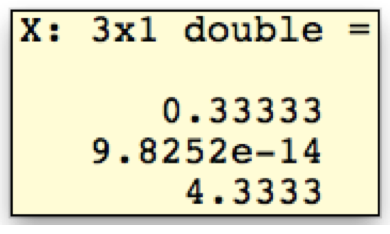
\includegraphics[width=3cm,height=2cm]{resp_minimizacao.png}
		\end{column}


	\end{columns}
\end{frame}